\documentclass[12pt,twoside]{article}

\addtolength{\textwidth}{0.5in}
\usepackage{epsfig,amsfonts,color}
%\usepackage[leqno]{amsmath}
\usepackage{amsmath}
%\usepackage{showlabels}
\newcommand{\norm}[1]{\left| \left| #1 \right| \right|}
\newcommand{\mods}[1]{\left|  #1 \right|}
\newcommand{\cm}[1]{{\color{black} #1}}
\newcommand{\cv}[1]{{\color{black} #1}}
\bibliographystyle{plain}
\usepackage{amssymb, palatino, geometry,url}
\usepackage{algorithmic}
\usepackage[noresetcount,lined,boxed]{algorithm2e} % ... for algorithms
\newcommand{\mynote}[1]{{ \color{black}{#1}}}
\usepackage[colorlinks=true,linkcolor=blue,citecolor=blue,urlcolor=blue]{hyperref}

\usepackage{multirow}

\geometry{letterpaper,
          left       = 0.9in,
          right      = 0.9in,
          top        = 0.9in,
          bottom     = 0.9in}
\linespread{1.2}

\usepackage{fancyhdr}
\pagestyle{fancy}

%\usepackage{lineno}
%\linenumbers

% Customize spacing in lists
\usepackage{enumitem}

% Globally set noindent
\setlength{\parindent}{0pt}

% Use to white out portion students will fill in

\newcommand{\fillin}[1]{{\color{white} \large #1}}

% For subfigures
\usepackage{graphicx}
\usepackage{caption}
\usepackage{subcaption}

% For floatbarrier
\usepackage{placeins}

% Check list
\newlist{todolist}{itemize}{2}
\setlist[todolist]{label=$\square$}

% Comments
\usepackage{verbatim}

\usepackage{tcolorbox}

\usepackage{mhchem}

% With subsections to alphabetical labeling
\renewcommand{\thesubsection}{\thesection.\alph{subsection}}

\newcommand{\assignmentname}{Error Propagation Example}

\lhead{\assignmentname}
\rhead{A.~Dowling, University of Notre Dame}

%\renewcommand\contentsname{Outline for Lecture X}

\title{\assignmentname}
\author{CBE 20258 / CBE 40258 / CBE 60258}


% define notation for vectors and matrix
% https://tex.stackexchange.com/questions/229543/double-tilde-symbol-under-letter
\usepackage{stackengine}
\stackMath
\newcommand\tenq[2][1]{%
 \def\useanchorwidth{T}%
  \ifnum#1>1%
    \stackunder[0pt]{\tenq[\numexpr#1-1\relax]{#2}}{\scriptscriptstyle\sim}%
  \else%
    \stackunder[1pt]{#2}{\scriptscriptstyle\sim}%
  \fi%
}

% Vector
\newcommand{\vc}[1]{\tenq{#1}}

% Matrix
\newcommand{\mt}[1]{\tenq[2]{#1}}


% Enable solutions
\usepackage{comment}
\specialcomment{sln}{\begingroup\color{red} \vspace{6pt} \textbf{Solution}: \vspace{6pt} \\}{\endgroup%\vfill\pagebreak
}

\newcommand{\ad}{\vspace{6pt}\textbf{Additional Discussion}:\vspace{6pt}}

% Number equations within subsection
% \numberwithin{equation}{section}

% Hide solutions
\excludecomment{sln}

% Expected value
\DeclareRobustCommand{\bbone}{\text{\usefont{U}{bbold}{m}{n}1}}

\DeclareMathOperator{\EX}{\mathbb{E}}% expected value
\DeclareMathOperator{\PR}{\mathbb{P}}% probability
\DeclareMathOperator{\VR}{\mathbb{V}}% variance

\usepackage{wrapfig}

\begin{document}

%\tableofcontents

\date{November 5, 2019}

% \maketitle

%%%%%%%%%%%%%%%%%%

\maketitle

\section{Experimental Setup}

\begin{wrapfigure}{R}{0.3\textwidth}
	\centering
	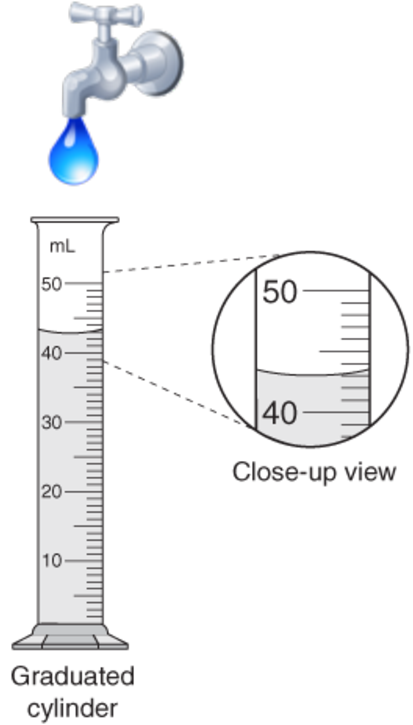
\includegraphics[width=0.25\textwidth]{experiment}
\end{wrapfigure}

Imagine you want to measure the flow rate of water out of a faucet, but your flowmeter is broken. Quick on your feet, you devise a simple experiment using a graduate cylinder and wrist watch. The average flow rate is:

\begin{equation}
	F = \frac{V_{f} - V_{0}}{t_{f} - t_{0}} \label{eq:main}
\end{equation}

where $V_{0}$ is the volume in the cylinder at time $t_{0}$. You measure $V_{f}$ and $t_f$ after some time has elapsed.

\section{Error Propagation}

Your graduated cylinder only measures to the nearest 0.1 mL and holds a maximum of 50 mL. Your analog wristwatch has a seconds hand. Based on this, you reason that $\sigma_V = $ \underline{\fillin{0.1}} mL (same for both volume measurements), $\sigma_t$ = \underline{\fillin{~1~}} s (same for both time measurements), and $\sigma_{V,t} =$ \underline{\fillin{~0~}} (i.e., the measurement errors are NOT correlated). Although you \emph{could} conduct many experiments to estimate $\sigma_V$, $\sigma_t$, and $\sigma_{V,t}$, you think it is wise to \emph{approximate} the error level in $F$ after taking only a few measurements. Here are the data for your first trial:

\begin{center}
\begin{tabular}{c c c c}
$V_{0}$ & $t_{0}$ & $V_{f}$ & $t_{f}$ \\ \hline
5.3 mL & 1:01:04 & 49.2 mL & 1:01:56 \\	
\end{tabular}
\end{center}

\vfill \pagebreak

\subsection{Approach 1}

Which error propagation formula to use? You decide to decompose \eqref{eq:main} into two subtraction steps and one division step:

\begin{equation}
	\Delta t := t_{f} - t_{0}, \qquad \Delta V := V_{f} - V_{0}, \qquad F = \frac{\Delta V}{\Delta t}
\end{equation}

where $\Delta V$ and $\Delta t$ are intermediate variables. You then apply the \underline{subtraction} error propagation formula to calculate $\sigma_{\Delta V}$ and $\sigma_{\Delta t}$.

\fillin{

\begin{equation*}
\sigma_{\Delta V} = \sqrt{\sigma_{V}^2 + \sigma_V^2} = \sqrt{2} ~ \sigma_{V}
\end{equation*}

\begin{equation*}
\sigma_{\Delta t} = \sqrt{\sigma_{t}^2 + \sigma_t^2} = \sqrt{2} ~ \sigma_{t}
\end{equation*}

}

\vspace{0.1\textheight}

Next, apply the \underline{division} error propagation formula to estimate $\sigma_F$:

\fillin{

\begin{align*}
\sigma_{F}^2 & \approx F^2 \left[ \left(\frac{\sigma_{\Delta V}}{\Delta V} \right)^2	+ \left(\frac{\sigma_{\Delta t}}{\Delta t} \right)^2 \right] \\
			& \approx F^2 \left[ 2 \left(\frac{\sigma_{V}}{\Delta V} \right)^2	+ 2 \left(\frac{\sigma_{t}}{\Delta t} \right)^2 \right]
\end{align*}

}

\vspace{0.1\textheight}

\vfill \pagebreak

\subsection{Approach 2}

What about the general error propagation formula,

\begin{equation}
	\sigma_Z^2 \approx \left| \frac{\partial g}{\partial X} \right|^2 \cdot \sigma_X^2 + \left| \frac{\partial g}{\partial Y} \right|^2 \cdot \sigma_Y^2 + 2 \cdot \frac{\partial g}{\partial X} \cdot \frac{\partial g}{\partial Y} \cdot \sigma_{X,Y} \label{eq:general_formula}
\end{equation}

where $Z = g(X,Y)$ and $g(\cdot)$ is a differentiable function? You apply this formula to \eqref{eq:main}. Start by calculating the partial derivatives $\frac{\partial F}{\partial V_{f}}$, $\frac{\partial F}{\partial V_{0}}$, $\frac{\partial F}{\partial t_{f}}$, $\frac{\partial F}{\partial t_{0}}$:

\fillin{

\begin{equation*}
	\frac{\partial F}{\partial V_f} = \frac{1}{t_f - t_{0}}
\end{equation*}

\begin{equation*}
	\frac{\partial F}{\partial V_{0}} = \frac{-1}{t_f - t_{0}}
\end{equation*}

\begin{equation*}
	\frac{\partial F}{\partial t_f} = - \frac{V_f - V_0}{(t_f - t_{0})^2}
\end{equation*}

\begin{equation*}
	\frac{\partial F}{\partial t_{0}} = \frac{V_f - V_{0}}{(t_f - t_{0})^2}
\end{equation*}

}

\vspace{0.05\textheight}

Next, apply the general formula, \eqref{eq:general_formula}, and drop the covariance terms (assumed to be zero).

\begin{equation*}
	\sigma_F^2 \approx \left| \frac{\partial F}{\partial V_{f}} \right|^2 \sigma_V^2 
						+ \left| \frac{\partial F}{\partial V_{0}} \right|^2 \sigma_V^2
						+ \left| \frac{\partial F}{\partial t_f} \right|^2 \sigma_t^2
						+ \left| \frac{\partial F}{\partial t_0} \right|^2 \sigma_t^2
\end{equation*}

Finally, substitute and simplify:

\fillin{
\begin{align*}
	\sigma_F^2 & \approx \left| \frac{1}{t_f - t_{0}} \right|^2 \sigma_V^2 
						+ \left| \frac{-1}{t_f - t_{0}} \right|^2 \sigma_V^2
						+ \left| - \frac{V_f - V_0}{(t_f - t_{0})^2} \right|^2 \sigma_t^2
						+ \left| \frac{V_f - V_{0}}{(t_f - t_{0})^2} \right|^2 \sigma_t^2 \\
			& \approx 2 \left( \frac{1}{t_f - t_{0}} \right)^2 \sigma_V^2 + 2 \left( \frac{V_f - V_{0}}{(t_f - t_{0})^2} \right)^2 \sigma_t^2 \\
			& \approx 2 \left( \frac{1}{\Delta t} \right)^2 \sigma_V^2 + 2 \left( \frac{\Delta V}{(\Delta t)^2} \right)^2 \sigma_t^2 \\
			& \approx \left(\frac{\Delta V}{\Delta t} \right)^2 \left[ 2 \left(\frac{\sigma_V}{\Delta V} \right)^2 + 2 \left(\frac{\sigma_t}{\Delta t} \right)^2 \right] \\
			& \approx F^2 \left[ 2 \left(\frac{\sigma_V}{\Delta V} \right)^2 + 2 \left(\frac{\sigma_t}{\Delta t} \right)^2 \right]
\end{align*}

\vfill \pagebreak

}

\section{Calculation}

Now that we have confirmed Approach 1 and Approach 2 yield the same error propagation formula, we can perform the calculation. Recall the data for the first trial:

\begin{center}
\begin{tabular}{c c c c}
$V_{0}$ & $t_{0}$ & $V_{f}$ & $t_{f}$ \\ \hline
5.3 mL & 1:01:04 & 49.2 mL & 1:01:56 \\	
\end{tabular}
\end{center}

and our assumptions $\sigma_V = 0.1$ mL and $\sigma_t$ = 1 s. \\

Calculate $F$ and estimate $\sigma_F$:

\begin{equation*}
	F = \frac{\Delta V}{\Delta t}, \qquad \sigma_{F}^2 \approx F^2 \left[ 2 \left(\frac{\sigma_{V}}{\Delta V} \right)^2	+ 2 \left(\frac{\sigma_{t}}{\Delta t} \right)^2 \right]
\end{equation*}

\fillin{

\begin{gather*}
\Delta V = V_f - V_0 = 49.2 - 5.3 = 43.9 \mathrm{~mL} \\
\Delta t = t_f - t_0 = 56 - 4 = 52 \mathrm{~s} \\
F = 0.8442 \mathrm{~ mL/s}	\\
\sigma_F \approx \left| F \right| \sqrt{2 \left(\frac{\sigma_{V}}{\Delta V} \right)^2	+ 2 \left(\frac{\sigma_{t}}{\Delta t} \right)^2} \approx 0.0231 \mathrm{~mL/s}
\end{gather*}

}

\end{document}
